%\chapter{Making NN's Work}
\section{Training}
Here we go!  Here's how to do stochastic gradient descent training on
a feed-forward neural network.\index{neural network!training}   After this pseudo-code, we motivate
the choice of initialization in lines 2 and 3.  The actual
computation of the gradient values (e.g., $\partial\text{loss}/
  \partial A^L$) is not directly defined in this code, because we want
to make the structure of the computation clear.
\question{What is $\partial Z^l / \partial W^l$? }
\question{Which terms in the code below depend on $f^L$?}

\begin{codebox}
  \Procname{$\proc{SGD-Neural-Net}(\dataTrain, T, L, (m^1, \ldots,
    m^L), (f^1, \ldots, f^L), \text{Loss})$}
    \li     \For $l \gets 1$ \To $L$
    \Do
    \li        $W_{ij}^l \sim \text{Gaussian}(0, 1/m^l)$
    \li        $W_{0j}^l \sim \text{Gaussian}(0, 1)$
    \End
    \li \For $t \gets 1$ \To $T$
    \li   \Do
  $i \gets \text{random sample from } \{1,\ldots,n\}$
    \li     $A^0 \gets \ex{x}{i}$
    \li     \Comment forward pass to compute the output $A^L$
    \li     \For $l \gets 1$ \To $L$
    \li       \Do
  $Z^l \gets W^{l^T}A^{l-1} + W_0^l$
    \li         $A^l \gets f^l(Z^l)$
    \End
    \li     $\text{loss} \gets \text{Loss}(A^L, \ex{y}{i})$
    \li     \For $l \gets L$ \To 1:
    \Do
    \li       \Comment error back-propagation
    \li       $\partial \text{loss}/\partial A^l \gets$ 	%
    %            m x 1
    {\bf if} $l < L$
    {\bf then}
    % dims:          n x 1                    *    m x n
  $\partial Z^{l+1}/\partial A^l \cdot \partial \text{loss}/\partial Z^{l+1} $
    % dims:  m x n                   *     n x 1
    {\bf else}
  $ \partial \text{loss}/\partial A^L$
    \li       $\partial \text{loss}/\partial Z^l \gets \partial
  A^l/\partial Z^l  \cdot \partial
  \text{loss}/\partial A^l$
    \li       \Comment compute gradient with respect to weights
    \li       $\partial \text{loss}/\partial W^l  \gets        A^{l-1}      \cdot    \left( \partial \text{loss}/\partial Z^l  \right)^T $
    %                           m x n              =            m x 1          *        1 x n
    \li       $\partial \text{loss}/\partial W_0^l \gets       \partial \text{loss}/\partial Z^l $
    %                           1 x n              =                  1 x n
    \li       \Comment stochastic gradient descent update
    \li       $W^l = W^l - \eta(t)\cdot \partial \text{loss}/\partial W^l$
    \li       $W^l_0 = W_0^l - \eta(t)\cdot \partial \text{loss}/\partial W_0^l$
  \End
\end{codebox}

Initializing $W$ is important;\index{neural network!initialization of weights}  if you do it badly there is a good
chance the neural network training won't work well.  First, it is
important to initialize the weights to random values.  We want
different parts of the network to tend to ``address'' different
aspects of the problem; if they all start at the same weights, the
symmetry will often keep the values from moving in useful directions.
Second, many of our activation functions have (near) zero slope when
the pre-activation $z$ values have large magnitude, so we generally
want to keep the initial weights small so we will be in a situation
where the gradients are non-zero, so that gradient descent will have
some useful signal about which way to go.

One good general-purpose strategy is to choose each weight at random
from a Gaussian (normal) distribution with mean 0 and standard
deviation $(1/m)$ where $m$ is the number of inputs to the unit.
\question{If the input $x$ to this unit is a vector of 1's, what would
  the expected pre-activation $z$ value be with these initial
  weights?}  We write this choice (where $\sim$ means ``is drawn
randomly from the distribution'') as $W^l_{ij} \sim \text{Gaussian}\left(0,
  \frac{1}{m^l}\right).$ It will often turn out (especially for fancier activations and loss
functions) that computing
$\frac{\partial \text{loss}}{\partial Z^L}$ is easier than computing
$\frac{\partial \text{loss}}{\partial A^L}$ and $\frac{\partial A^L}{\partial Z^L}.$ So, we may instead ask for an implementation of a loss function to provide a backward method that computes $\partial \text{loss}/\partial Z^L$ directly.


\section{Optimizing neural network parameters}
\label{sec-make_nn_work}

Because neural networks are just parametric functions, we can optimize
loss with respect to the parameters using standard gradient-descent
software, but we can take advantage of the structure of the loss
function and the hypothesis class to improve optimization.  As we have
seen, the modular function-composition structure of a neural network
hypothesis makes it easy to organize the computation of the gradient.
As we have also seen earlier, the structure of the loss function as a
sum over terms, one per training data point, allows us to consider
stochastic gradient methods.  In this section we'll consider some
alternative strategies for organizing training, and also for making it
easier to handle the step-size parameter.

\subsection{Batches}
Assume that we have an objective of the form
\[J(W) = \sum_{i = 1}^n \mathcal{L}(h(\ex{x}{i}; W),  \ex{y}{i})\;\;,\]
where $h$ is the function computed by a neural network, and $W$ stands
for all the weight matrices and vectors in the network.

When we perform {\em batch} gradient descent, we use the update rule
\[W_t = W_{t-1} - \eta\nabla_W J(W_{t-1})\;\;,\]
which is equivalent to
\[W_t = W_{t-1} - \eta\sum_{i=1}^n \nabla_W \mathcal{L}(h(\ex{x}{i}; W_{t-1}),
  \ex{y}{i})\;\;.\]
So, we sum up the gradient of loss at each training point,  with
respect to $W$, and then take a step in the negative direction of
the gradient.

In {\em stochastic} gradient descent, we repeatedly pick a point
$(\ex{x}{i}, \ex{y}{i})$ at random from the data set, and execute a
weight update on that point alone:
\[W_t = W_{t-1} - \eta \nabla_W \mathcal{L}(h(\ex{x}{i}; W_{t-1}),
  \ex{y}{i})\;\;.\]
As long as we pick points uniformly at random from the data set, and
decrease $\eta$ at an appropriate rate, we are guaranteed, with high
probability, to converge to at least a local optimum.

These two methods have offsetting virtues.  The batch method takes
steps in the exact gradient direction but requires a lot of
computation before even a single step can be taken, especially if the
data set is large.  The stochastic method begins moving right away,
and can sometimes make very good progress before looking at even a
substantial fraction of the whole data set, but if there is a lot of
variability in the data, it might require a very small $\eta$ to
effectively average over the individual steps moving in ``competing''
directions.

An effective strategy is to ``average'' between batch and stochastic
gradient descent by using {\em mini-batches}.  For a mini-batch of
size $K$, we select $K$ distinct data points uniformly at random from the data
set and do the update based just on their contributions to the gradient
\[W_t = W_{t-1} - \eta\sum_{i=1}^K \nabla_W \mathcal{L}(h(\ex{x}{i}; W_{t-1}),
  \ex{y}{i})\;\;.\]
Most neural network software packages are set up to do mini-batches.
\question{For what value of $K$ is mini-batch gradient descent
  equivalent to stochastic gradient descent?  To batch gradient
  descent?}

Picking $K$ unique data points at random from a large data-set is
potentially computationally difficult.  An alternative strategy, if
you have an efficient procedure for randomly shuffling the data set
(or randomly shuffling a list of indices into the data set) is to
operate in a loop, roughly as follows:

\begin{codebox}
  \Procname{$\proc{Mini-Batch-SGD}$(NN, data, K)}
  \li     $n = $ length(data)
  \li     \While not done:
  \Do
  \li        $\proc{Random-Shuffle}$(data)
  \li        \For $i \gets 1$ \To $\lceil n/K \rceil$
  \Do
  \li           $\proc{Batch-Gradient-Update}$(NN, data$[(i - 1)K:iK]$)
  \End
  \End
\end{codebox}
See note on the ceiling\footnote{
  In line 4 of the algorithm above, $\lceil \cdot \rceil$ is known
  as the \emph{ceiling} function; it returns the smallest
  integer greater than or equal to its input. E.g., $\lceil 2.5 \rceil = 3$ and $\lceil 3 \rceil = 3$.}
function, for the case when $n/K$ is not an integer.

\subsection{Adaptive step-size}
Picking a value for $\eta$ is difficult and time-consuming.\index{adaptive step size}  If it's
too small, then convergence is slow and if it's too large, then we
risk divergence or slow convergence due to oscillation.  This problem
is even more pronounced in stochastic or mini-batch mode, because we
know we need to decrease the step size for the formal guarantees to
hold.

It's also true that, within a single neural network, we may well want
to have different step sizes.  As our networks become {\em deep} (with
increasing numbers of layers) we can find that magnitude of the
gradient of the loss with respect the weights in the last layer,
$\partial \text{loss} / \partial W_L$, may be substantially
different from the gradient of the loss with respect to the weights in
the first layer $\partial \text{loss} / \partial W_1$.  If you look
carefully at Eq.~\ref{eq:gradz}, you can see that the output
gradient is multiplied by all the weight matrices of the network and
is ``fed back'' through all the derivatives of all the activation
functions.  This can lead to a problem of {\em exploding}  or {\em
    vanishing} gradients\index{exploding (or vanishing) gradients}, in which the back-propagated gradient is much
too big or small to be used in an update rule with the same step size.

So, we'll consider having an independent step-size parameter {\em for each
    weight}, and updating it based on a local view of how the gradient
updates have been going.\note{This section is very strongly influenced
by Sebastian Ruder's excellent blog posts on the topic:
{\tt\scriptsize ruder.io/ optimizing-gradient-descent}}

\subsubsection{Running averages}
\index{adaptive step size!running average}
We'll start by looking at the notion of a {\em running average}.  It's
a computational strategy for estimating a possibly weighted average of
a sequence  of data.  Let our data sequence be $a_1, a_2, \ldots$;
then we define a sequence of running average values, $A_0, A_1, A_2,
  \ldots$ using the equations
\begin{align*}
  A_0 & = 0                                       \\
  A_t & =  \gamma_t A_{t-1} +  (1 - \gamma_t) a_t
\end{align*}
where $\gamma_t \in (0, 1)$.  If $\gamma_t$ is a constant, then this
is a {\em  moving} average, in which
\begin{align*}
  A_T & = \gamma A_{T-1} + (1  - \gamma) a_T                                  \\
      & = \gamma (\gamma A_{T-2} + (1  - \gamma) a_{T-1}) + (1  - \gamma) a_T \\
      & = \sum_{t = 1}^T \gamma^{T-t}(1 - \gamma) a_t
\end{align*}
So, you can see that inputs $a_t$ closer to the end of the sequence $T$
have  more effect on $A_T$ than early inputs.

If, instead, we set $\gamma_t = (t - 1)  / t$, then we get the actual
average.
\question{
  Prove to yourself that the previous assertion holds.
}
% \begin{align*}
% A_1 &= a_1\\
% A_2 &= \frac{1}{2}A_1 + \frac{1}{2}a_2 = \frac{1}{2}(a_1 + a_2)\\
% A_3 &= \frac{2}{3}A_2 + \frac{1}{3}a_3 = \frac{2}{3} \cdot \frac{1}{2}(a_1 + a_2) + \frac{1}{3}a_3 = \frac{1}{3}(a_1 + a_2 + a_3)
% \end{align*}

\subsubsection{Momentum} \index{adaptive step size!momentum}
Now, we can use methods that are a bit like running averages to
describe strategies for computing $\eta$.
The simplest method is {\em momentum}, in  which we try to ``average'' recent
gradient updates,  so that if they have been bouncing back and forth
in some direction, we take out that component of the motion.  For
momentum, we have
\begin{align*}
  V_0 & = 0                                         \\
  V_t & = \gamma V_{t-1} + \eta \nabla_W J(W_{t-1}) \\
  W_t & = W_{t-1} - V_t
\end{align*}
This doesn't quite look like an adaptive step size.  But what we can
see is that, if we let $\eta = \eta'(1 - \gamma)$, then the rule looks exactly like doing an update with
step size $\eta'$ on a moving average of the gradients with parameter
$\gamma$:
\begin{align*}
  M_0 & = 0                                                 \\
  M_t & = \gamma M_{t-1} + (1 - \gamma) \nabla_W J(W_{t-1}) \\
  W_t & = W_{t-1} - \eta' M_t
\end{align*}
\question{Prove to yourself that these formulations are equivalent.}


We will find that $V_t$ will be bigger in dimensions that consistently
have the same sign for $\nabla_{W}$ and smaller for those that
don't.   Of course we now have {\em two}  parameters  to set ($\eta$
and $\gamma$), but the
hope is  that the algorithm will perform better overall, so it will be
worth trying to find good values for them.  Often $\gamma$ is  set to
be something like $0.9$.
\begin{examplebox}
  \begin{center}
    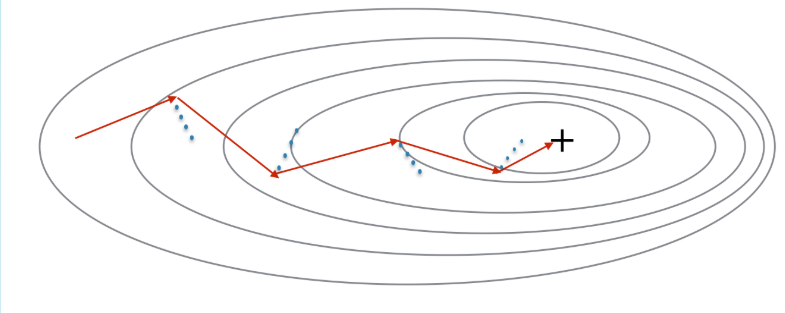
\includegraphics[scale=0.7]{figures/momentum.png}
  \end{center}
  The red arrows show the update after each successive step of
  mini-batch gradient descent with momentum.  The blue points show the
  direction of the gradient with respect to the mini-batch at each step.
  Momentum smooths the path taken towards the local minimum and leads to
  faster convergence.
\end{examplebox}
\question{If you set $\gamma = 0.1$, would momentum have more of an
  effect or less of an effect than if you set it to $0.9$?
}

\subsubsection{Adadelta}\index{adaptive step size!adadelta}
Another useful idea is this:  we would like to take larger steps in
parts of the space where $J(W)$ is nearly flat (because there's no risk of
taking too big a step due to the gradient being large) and smaller
steps when it is steep.  We'll apply this idea to each weight
independently, and end up with a method called {\em adadelta}, which
is a variant on {\em adagrad} (for
adaptive gradient).   Even though our weights are indexed by layer,
input unit and output unit,  for simplicity here,  just let $W_j$ be
any weight in the network (we will do the same thing for all of
them).
\begin{align*}
  g_{t,j} & = \nabla_W J(W_{t-1})_j                                      \\
  G_{t,j} & = \gamma G_{t - 1,j} + (1 - \gamma)g_{t,j}^2                 \\
  W_{t,j} & = W_{t-1, j} - \frac{\eta}{\sqrt{G_{t,j} + \epsilon}}g_{t,j}
\end{align*}
The sequence $G_{t,j}$ is a moving average of the  square of the
$j$th component of the gradient.  We square it in order to be
insensitive to the sign---we want to know whether the magnitude is big
or small.  Then, we perform a gradient update to weight $j$, but
divide the step  size by $\sqrt{G_{t,j} + \epsilon}$, which is larger
when the surface is steeper in direction $j$ at point $W_{t-1}$ in
weight space;  this means that the step size will be smaller when it's
steep and  larger when it's flat.

\subsubsection{Adam}\index{adaptive step size!adam}

Adam has become the default method of managing step sizes in neural
networks\note{Although,  interestingly, it may actually violate the
convergence conditions of {\sc sgd}: {\scriptsize\tt
arxiv.org/abs/1705.08292}}.   It combines the ideas  of
momentum and adadelta.  We start by writing moving averages of the
gradient and squared gradient, which reflect estimates of the mean and
variance of the gradient for weight $j$:
\begin{align*}
  g_{t,j} & = \nabla_W J(W_{t-1})_j                      \\
  m_{t,j} & = B_1m_{t - 1,j} + (1 - B_1)g_{t,j}          \\
  v_{t,j} & = B_2v_{t - 1,j} + (1 - B_2)g_{t,j}^2  \;\;.
\end{align*}

A problem with these estimates is that, if we initialize $m_0 = v_0 = 0$,
they will always be biased (slightly too small).  So we will correct
for that bias  by defining
\begin{align*}
  \hat{m}_{t,j} & = \frac{m_{t,j}}{1 - B^t_1}                     \\
  \hat{v}_{t,j} & = \frac{v_{t,j}}{1 - B^t_2}                     \\
  W_{t,j}       & = W_{t-1,j} - \frac{\eta}{\sqrt{\hat{v}_{t,j} +
      \epsilon}}\hat{m}_{t,j} \;\;.
\end{align*}
Note that $B^t_1$ is $B_1$ raised to the power $t$, and likewise for
$B^t_2$.  To justify these corrections, note that if we were to expand $m_{t,j}$
in terms of $m_{0,j}$ and $g_{0,j}, g_{1,j}, \dots, g_{t,j}$ the coefficients would
sum to $1$.  However, the coefficient behind $m_{0,j}$ is $B_1^t$ and since
$m_{0,j} = 0$, the sum of coefficients of non-zero terms is $1 - B_1^t$, hence
the correction.  The same justification holds for $v_{t,j}$.

Now, our update for weight $j$ has a step size that takes the
steepness into account, as in adadelta, but also tends to move in the
same direction, as in momentum.  The authors of this method propose
setting $B_1 = 0.9, B_2 = 0.999, \epsilon = 10^{-8}$.  Although we now
have even more parameters, Adam is not highly sensitive to their values
(small changes do not have a huge effect on the result).
\question{Define $\hat{m_j}$ directly as a moving average of
  $g_{t,j}$.  What is the decay ($\gamma$ parameter)?
}
Even though we now have a step-size for each weight, and we have to
update various quantities on each iteration of gradient descent, it's
relatively easy to implement by maintaining a matrix for each quantity
($ m^{\ell}_t, v^{\ell}_t, g^{\ell}_t, {g^{2}_t}^{\ell} $) in each
layer of the network.

\section{Regularization}\index{neural network!regularization}
So far, we have only considered optimizing loss on the training data
as our objective for neural network training.   But, as we have
discussed before, there is a risk of overfitting if we do this.  The
pragmatic fact is that,  in current deep neural networks, which tend to be very
large and to be trained with a large amount of data,  overfitting is
not a huge problem.  This runs counter to our current theoretical
understanding and the study of this question is a hot area of
research.  Nonetheless, there are several strategies for regularizing
a neural network, and they can sometimes be important.

\subsection{Methods related to ridge regression}

One group of strategies can, interestingly, be shown to have similar
effects to each other: early stopping, weight decay, and adding noise
to the training data. \note{Result is due to Bishop, described in his
  textbook and here {\tt\scriptsize doi.org/10.1162/ neco.1995.7.1.108}.}

Early stopping is the easiest to implement and is in fairly common
use.  The idea is to train on your training set, but at every {\em
    epoch} (a pass through the whole training set, or possibly more
frequently), evaluate the loss of the current $W$ on a {\em validation
    set}.  It will generally be the case that the loss on the training
set goes down fairly consistently with each iteration, the loss on the
validation set will initially decrease, but then begin to increase
again.  Once you see that the validation loss is systematically
increasing, you can stop training and return the weights that had the
lowest validation error.

Another common strategy is to simply penalize the norm of all the
weights, as we did in ridge regression.  This  method is known as {\em
    weight decay}\index{neural network!weight decay}, because when we take the gradient of the objective
$$ J(W) = \sum_{i = 1}^{n}\mathcal{L}(\text{NN}(x^{(i)}), y^{(i)}; W)
  + \lambda\|W\|^2 $$
we end up  with an update of the form
\begin{align*}
  W_t & = W_{t-1} -
  \eta\left(\left(\nabla_{W}\mathcal{L}(\text{NN}(x^{(i)}),
  y^{(i)}; W_{t-1})\right) + 2\lambda W_{t-1}\right)                                      \\
      & = W_{t-1}(1 - 2\lambda\eta) - \eta\left(\nabla_{W}\mathcal{L}(\text{NN}(x^{(i)}),
    y^{(i)}; W_{t-1})\right) \;\;.
\end{align*}
This rule has the form of first ``decaying'' $W_{t-1}$ by a factor of
$(1 - 2 \lambda \eta)$ and then taking a gradient step.

Finally, the same effect can be achieved by perturbing the $\ex{x}{i}$
values of the training data by adding a small amount of zero-mean
normally distributed noise before each gradient computation.  It makes
intuitive sense that it would be more difficult for the network to
overfit to particular training data if they are changed slightly on
each training step.

\subsection{Dropout}
Dropout\index{neural network!dropout} is a regularization method that was designed to work with deep
neural networks.  The idea behind it is, rather than perturbing the
data every time we train, we'll perturb the network!  We'll do this by
randomly, on each training step, selecting a set of units in each
layer and prohibiting them from participating.   Thus, all of the
units will have to take a kind of  ``collective'' responsibility for
getting the answer right, and will not be able to rely on any small
subset of the weights to do all the necessary computation.  This tends
also to make the network more robust to data perturbations.

During the training phase, for each training example, for each unit,
randomly with probability $p$ temporarily set $a^{\ell}_j = 0$. There
will be no contribution to the output and no gradient update for the
associated unit.
\question{
  Be sure you understand why, when using {\sc sgd}, setting an
  activation value to 0 will cause that unit's weights not to be updated
  on that iteration.
}

When we are done training and want to use the network to make
predictions, we multiply all weights by $p$ to achieve the same average
activation levels.

Implementing dropout is easy!  In the forward pass during training, we let
$$ a^{\ell} = f(z^{\ell}) * d^{\ell} $$
where $*$ denotes component-wise product and $d^{\ell}$ is a vector of
$0$'s and $1$'s drawn randomly with probability $p$.
The backwards pass depends on $a^{\ell}$, so we do not need to make
any further changes to the algorithm.

It is common to set $p$ to $0.5$, but this is something one might
experiment with to get good results on your problem and data.

% Dropout is no longer in common use, but it is still interesting to
% think about.

\subsection{Batch normalization}

Another strategy that seems to help with regularization and robustness
in training is {\em batch normalization}.  \index{neural network!batch normalization}
\note{For more  details see {\tt\scriptsize arxiv.org/abs/1502.03167}.}
It was originally
developed to address a problem of {\em covariate shift}:  that is, if
you consider the second layer of a two-layer neural network, the
distribution of its input values is changing over time as the first
layer's  weights change.  Learning when the input distribution is
changing is extra difficult:  you have to change your weights to
improve your predictions, but also just to compensate for a change in
your inputs  (imagine, for instance, that the magnitude of the inputs
to your layer is increasing over time---then your weights will have to
decrease, just to keep your predictions the same).

So, when training with mini-batches, the idea is to {\em standardize}
the input values for each mini-batch, just in the way that we did it
in Section~\ref{realFeatures} of Chapter~\ref{chap-features}, subtracting off the mean
and dividing by the standard deviation of each input dimension.  This
means that the scale of the inputs to each layer remains the same, no
matter how the weights in previous layers change.  However, this
somewhat complicates matters, because the computation of the weight
updates will need to take into account that we are performing this
transformation.  In the modular view, batch normalization can be seen
as a module that is applied to $z^l$, interposed after the product
with $W^l$ and before input to $f^l$.\note{We follow here the
  suggestion from the original paper of applying batch normalization
  before the activation function.  Since then it has been shown that,
  in some cases, applying it after works a bit better. But there
  aren't any definite findings on which works better and when.}

Although batch-norm was originally justified based on the problem of
covariate shift, it's not clear that that is actually why it seems to
improve performance.
Batch normalization can also end up having a regularizing effect for similar
reasons that adding noise and dropout do:  each mini-batch of data
ends up being mildly perturbed, which prevents the network from
exploiting very particular values of the data points.

Let's think of the batch-norm layer as taking $Z^l$ as input and
producing an output $\widehat{Z}^l$ as output.  But now, instead of
thinking of $Z^l$ as an $n^l \times 1$ vector, we have to explicitly
think about handling a mini-batch of data of size $K$, all at once, so
$Z^l$ will be $n^l \times K$, and so will the output $\widehat{Z}^l$.

Our first step will be to compute the {\em batchwise} mean and
standard deviation.  Let $\mu^l$ be the $n^l \times 1$ vector where
\[\mu^l_i = \frac{1}{K} \sum_{j = 1}^K Z^l_{ij}\;\;,\]
and let $\sigma^l$ be the $n^l \times 1$ vector where
\[\sigma^l_i = \sqrt{\frac{1}{K} \sum_{j = 1}^K (Z^l_{ij} - \mu_i)^2}\;\;.\]

The basic normalized version of our data would be a matrix,
element $(i, j)$ of which is
\[\overline{Z}^l_{ij} = \frac{Z^l_{ij} - \mu^l_i}{\sigma^l_i + \epsilon}\;\;,\]
where $\epsilon$ is a very small constant to guard against division by
zero.
However, if we let these be our $\widehat{Z}^l$ values, we really are
forcing something too strong on our data---our goal was to normalize
across the data batch, but not necessarily force the output values to
have exactly mean 0 and standard deviation 1.  So, we will give the
layer the ``opportunity'' to shift and scale the outputs by adding new
weights to the layer.  These weights are $G^l$ and $B^l$, each of
which is an $n^l \times 1$ vector.  Using the weights, we define the
final output to be
\[\widehat{Z}^l_{ij} = G^l_i \overline{Z}^l_{ij} + B^l_i\;\;.\]
That's the forward pass.  Whew!

Now, for the backward pass, we have to do two things:  given
$\partial L / \partial \widehat{Z}^l$,
\begin{itemize}
  \item Compute $\partial L / \partial Z^l$ for back-propagation, and
  \item Compute $\partial L / \partial G^l$ and $\partial L / \partial
          B^l$ for gradient updates of the weights in this layer.
\end{itemize}

Schematically\note{For simplicity we will drop the reference to the layer $l$ in the rest of the derivation}
\[\frac{\partial L}{\partial B} = \frac{\partial L}{\partial
    \widehat{Z}}\frac{\partial \widehat{Z}}{\partial B}\;\;.\]
It's hard to think about these derivatives in matrix terms, so we'll
see how it works for the components.
$B_i$ contributes to $\widehat{Z}_{ij}$ for all data points $j$ in the
batch.  So
\begin{align*}
  \frac{\partial L}{\partial B_i} & =
  \sum_j \frac{\partial L}{\partial \widehat{Z}_{ij}}
  \frac{\partial \widehat{Z}_{ij}}{\partial B_i}                                               \\
                                  & = \sum_j \frac{\partial L}{\partial \widehat{Z}_{ij}}\;\;,
\end{align*}
Similarly, $G_i$ contributes to $\widehat{Z}_{ij}$ for all data points
$j$ in the batch.  So
\begin{align*}
  \frac{\partial L}{\partial G_i} & =
  \sum_j \frac{\partial L}{\partial \widehat{Z}_{ij}}
  \frac{\partial \widehat{Z}_{ij}}{\partial G_i}                                                                  \\
                                  & =  \sum_j \frac{\partial L}{\partial \widehat{Z}_{ij}} \overline{Z}_{ij}\;\;.
\end{align*}
Now, let's figure out how to do backprop.  We can start schematically:
\[\frac{\partial L}{\partial Z} = \frac{\partial L}{\partial \widehat{Z}}
  \frac{\partial \widehat{Z}}{\partial Z}\;\;.\]
And because dependencies only exist across the batch, but not across
the unit outputs,
\[\frac{\partial L}{\partial Z_{ij}} =
  \sum_{k=1}^K\frac{\partial L}{\partial \widehat{Z}_{ik}}
  \frac{\partial \widehat{Z}_{ik}}{\partial Z_{ij}}\;\;.\]
The next step is to note that
\begin{align*}
  \frac{\partial \widehat{Z}_{ik}}{\partial Z_{ij}} & =
  \frac{\partial \widehat{Z}_{ik}}{\partial \overline{Z}_{ik}}
  \frac{\partial \overline{Z}_{ik}}{\partial Z_{ij}}                                                                \\
                                                    & = G_i \frac{\partial \overline{Z}_{ik}}{\partial Z_{ij}}\;\;.
\end{align*}
And now that
\[
  \frac{\partial \overline{Z}_{ik}}{\partial Z_{ij}}  =
  \left(\delta_{jk} - \frac{\partial \mu_i}{\partial Z_{ij}}\right) \frac{1}{\sigma_i} -
  \frac{Z_{ik} - \mu_i}{\sigma_i^2} \frac{\partial \sigma_i}{\partial Z_{ij}} \;\;,
\]
where $\delta_{jk} = 1$ if $j = k$ and $\delta_{jk} = 0$ otherwise.
Getting close!  We need two more small parts:
\begin{align*}
  \frac{\partial \mu_i}{\partial Z_{ij}}    & = \frac{1}{K} \;, \\
  \frac{\partial \sigma_i}{\partial Z_{ij}} & =
  \frac{Z_{ij} - \mu_i}{K \sigma_i}\;\;.
\end{align*}
Putting the whole crazy thing together, we get
\[\frac{\partial L}{\partial Z_{ij}} =
  \sum_{k=1}^K\frac{\partial L}{\partial \widehat{Z}_{ik}}
  G_i\frac{1}{K \sigma_i}\left(\delta_{jk}K-1 - \frac{(Z_{ik} - \mu_i)(Z_{ij} - \mu_i)}{\sigma_i^2}
  \right)\;\;.
\]


%%% Local Variables:
%%% mode: latex
%%% TeX-master: "top"
%%% End:
